\chapter{Computational Evidence Portfolio}
\label{ch:computation}

\section{Selection and evaluation rule}

This chapter reviews eight retained artifact families. Each entry records the
method, the paper-ready output it could support, one validation check, and the
strongest permissible inference. This format prevents an implementation check
from silently becoming a claim about nature.

\small
\begin{longtable}{>{\raggedright\arraybackslash}p{0.14\textwidth}
                  >{\raggedright\arraybackslash}p{0.26\textwidth}
                  >{\raggedright\arraybackslash}p{0.23\textwidth}
                  >{\raggedright\arraybackslash}p{0.20\textwidth}}
  \caption{Experiment artifacts, figure targets, and validation gates.}
  \label{tab:experiment-portfolio}\\
  \toprule
  Artifact & Method and figure target & Validation check & Permissible inference \\
  \midrule
  \endfirsthead
  \toprule
  Artifact & Method and figure target & Validation check & Permissible inference \\
  \midrule
  \endhead
  Fractal estimates &
    \path{experiments/results/fractal_dimensions.json}. Finite-resolution box
    counting or correlation sums. Plot fitted slope by
    scale with the selected window marked. &
    Repeat at increasing sample counts and shift the fit window. Compare with
    known dimensions. &
    Tests the estimator on selected synthetic sets. \\
  Modular forms &
    \path{experiments/results/modular_forms_analysis.json}. Truncated series
    evaluation. Plot absolute error for known special values
    against truncation order. &
    Verify $j(i)=1728$ and the zero at the cubic elliptic point to stated
    tolerance. &
    Checks numerical evaluation of standard identities. \\
  Cayley--Dickson &
    \path{experiments/results/cayley_dickson_real_validation.json}. Generated
    property record. A table reports finite identity checks by dimension. &
    Regenerate atomically, parse as JSON, and compare checks with direct
    calculations. &
    Finite computational checks of standard algebraic properties. \\
  E8 analysis &
    \path{experiments/results/e8_analysis.json}. Generated root-system summary.
    Plot root norms and pairwise inner-product
    multiplicities. &
    Parse the file, then test root count, rank, norms, opposite closure, and
    Cartan determinant against independent construction. &
    Finite validation of the generated $E_8$ root corpus. \\
  High-resolution LBM Parquet snapshots &
    BGK-style lattice-Boltzmann evolution with noise. Plot mass, momentum, and
    kinetic energy versus step before any spectrum. &
    Inspect schemas, prove fixed boundary and forcing conventions, and bound
    conservation drift. &
    Retained numerical trajectories, not beta-plane evidence. \\
  LBM demonstration &
    \path{experiments/quantum_lbm_stable_results.json}. A 32 by 32, 50-step
    conservation regression. Plot total mass and kinetic energy versus step. &
    Require relative mass drift below a prespecified tolerance. &
    The corrected CPU path conserves mass; it remains a numerical test, not
    evidence of quantum or exceptional-algebra dynamics. \\
  Layered harmonics &
    \path{experiments/data/genesis_harmonics_e7.json}. Deterministic layered
    frequencies and amplitudes. Plot amplitude against
    layer index with the generating formula. &
    Regenerate byte-equivalent output from a recorded version and seed. &
    Describes a chosen parameterization; it does not measure E7 physics. \\
  Generated registries &
    File discovery, size, and SHA-256 capture. Plot artifact counts by kind or
    use a compact inventory table. &
    Rebuild registries and verify every digest and schema. &
    Supports provenance and integrity only. \\
  \bottomrule
\end{longtable}

\section{Repaired result serialization}

The first audit found two experiment JSON files truncated inside scalar values.
That historical failure showed that registry inclusion checked identity but not
parseability. The current files are generated by
\path{scripts/generate_core_validation_results.py}, written atomically, parsed
by tests, and checked against explicit finite invariants. The E8 record now
contains 240 roots, 120 positive roots, rank 8, dimension 248, norm-squared
multiplicity 240 at value 2, opposite closure, and Cartan determinant 1. The
Cayley--Dickson record reports only properties actually calculated by its
generator.

\begin{evidence}{Repaired computational artifacts}
The files now support their stated finite checks. Repairing serialization does
not promote those checks into physical evidence, and future registry generation
still needs a general parse-and-schema gate rather than file existence alone.
\end{evidence}

\section{Fractal-dimension estimates}

The retained fractal result contains scales, measures, fitted dimensions,
regression errors, and coefficients of determination. This is a better evidence
shape than a single scalar. It still lacks a convergence study over resolution
and fit-window selection. For example, the retained Cantor-set estimate is
approximately $0.675$, while the exact middle-thirds value is
$\log 2/\log 3\approx0.631$. The discrepancy is large enough that the estimator
must be described as finite-resolution and method-dependent.

\begin{evidence}{Computational check}
The artifact can support a methods figure showing scale dependence. It cannot
support a claim that arbitrary framework geometries have a validated fractal
dimension.
\end{evidence}

\section{Modular-form special values}

The modular-form artifact records $j(i)=1728$ numerically and a near-zero value
at an approximation to the cubic elliptic point. It also records initial
coefficients of the $j$ expansion and Ramanujan tau values. These are useful
regression targets because independent reference values exist.

\begin{evidence}{Computational check}
Agreement verifies a limited numerical implementation. The computation contains
no data from a physical system and therefore supplies no evidence for a
moonshine-based physical mechanism.
\end{evidence}

\section{The CPU LBM defect and repair}

The first audit found that the file named
\texttt{quantum\_lbm\_stable\_results.json} grew from initial mass near
$1.024\times10^3$ to final mass near $1.251\times10^6$ after 50 steps. The
failure was not generic LBM instability. The CPU equilibrium used standard
D2Q9 coefficients and then divided by the sound-speed powers a second time.
At nonzero velocity its populations summed to $\rho(1+9|u|^2)$ rather than
$\rho$.

The equilibrium now uses the dimensionally consistent coefficient form. The
conservation validator measures relative error against initialized mass instead
of returning a constant verdict. The regenerated 50-step periodic run conserves
mass to approximately $1.78\times10^{-15}$ relative error. Tests also inject
mass deliberately and require the validator to reject the altered state.

\begin{evidence}{Repaired numerical regression}
The corrected result validates one conservation prerequisite for the CPU code.
The root-indexed initial condition and passive auxiliary arrays still supply no
evidence for quantum transport, coherent flow, or a cross-domain physical map.
\end{evidence}

\section{High-resolution snapshot mismatch}

The high-resolution driver leaves the requested harmonic count and Reynolds
metadata unchanged, giving 127 and 100 respectively. Only 126 E7 roots exist,
so the effective initializer count is 126; the Reynolds field does not enter
the evolution. The superseded paper assembly instead reported 10 harmonics and
Reynolds number 10. A direct read of the final Parquet snapshot
finds dominant zonal-mean mode 17, mean speed $6.92\times10^{-3}$, and maximum
speed $1.10\times10^{-2}$, not the published mode 4 and characteristic speed
0.6. The mode-17 zonal profile is weak: its RMS is $1.22\times10^{-3}$ of total
velocity RMS. A vorticity-power second-moment ratio of 0.992 is close to
isotropic. Relative mass drift rises smoothly to $5.60\times10^{-6}$ by step
500; this is measurable but not the catastrophic CPU failure. No checked-in
analysis computes the reported uncertainty or a $-5/3$ fit.

\begin{evidence}{Retained output contradicts the superseded claim}
Every reported table cell must be generated from a versioned analysis command
and stored beside the run parameters. Values that cannot be traced to that path
are removed rather than rounded into agreement.
\end{evidence}

\section{Resolved structural gate and controlled next experiment}

The exhaustive triad inventory closes the structural gate. The unique
nontrivial square-symmetry-invariant homomorphism from the Fourier lattice to
$P/Q\simeq\mathbb{Z}/2$ is $h(k_x,k_y)=k_x+k_y\pmod 2$. It admits every exact
triad by additivity, so the proposed filter equals its identity control before
any dynamics are run.

The short matched beta-plane ablation tests implementation sensitivity and
records the algebraic filter as a prespecified negative control. It is not the
scientific jet test. The production program separately executes 540 paired
runs across five beta values, three drag values, three viscosities, and twelve
independent seed clusters:

\begin{enumerate}
  \item implement the beta-dependent evolution independently of quotient labels;
  \item compare the homomorphic filter with its bit-identical identity control;
  \item specify mass, energy, enstrophy, anisotropy, and jet diagnostics before
    running;
  \item execute a committed-before-rerun resolution and time-step refinement study;
  \item report seed-clustered effect sizes and simultaneous uncertainty bounds;
  \item require zero filter effect to numerical precision and reject any claimed
    algebraic effect if the trajectories differ.
\end{enumerate}

The numerical, refinement, and control gates pass. The registered scientific
hypothesis does not. At $\beta=5$, the zonal-fraction effect is $-0.0030$ and
the persistent-jet-prevalence effect is $0.1019$. At $\beta=10$, the effects
are $-0.0200$ and $0.0000$. Every required simultaneous interval crosses zero,
and every required effect misses its locked minimum. An independent clean
container reproduces the negative aggregate decision. The result is evidence
against the declared transient-zonalization effect in this freely decaying
model; it is not evidence against beta-plane jet formation under other forcing
or dissipation regimes.

This experiment cannot rehabilitate the root-lattice interpretation. The first
nonhomomorphic candidate also fails specificity: its $E_7$ quadratic-defect
mask is exactly the generic even-checkerboard kernel at every enumerated triad.
Generic parity-kernel dynamics would define a different mechanism and still
requires conservation and matched-control gates.

\begin{figure}[htbp]
  \centering
  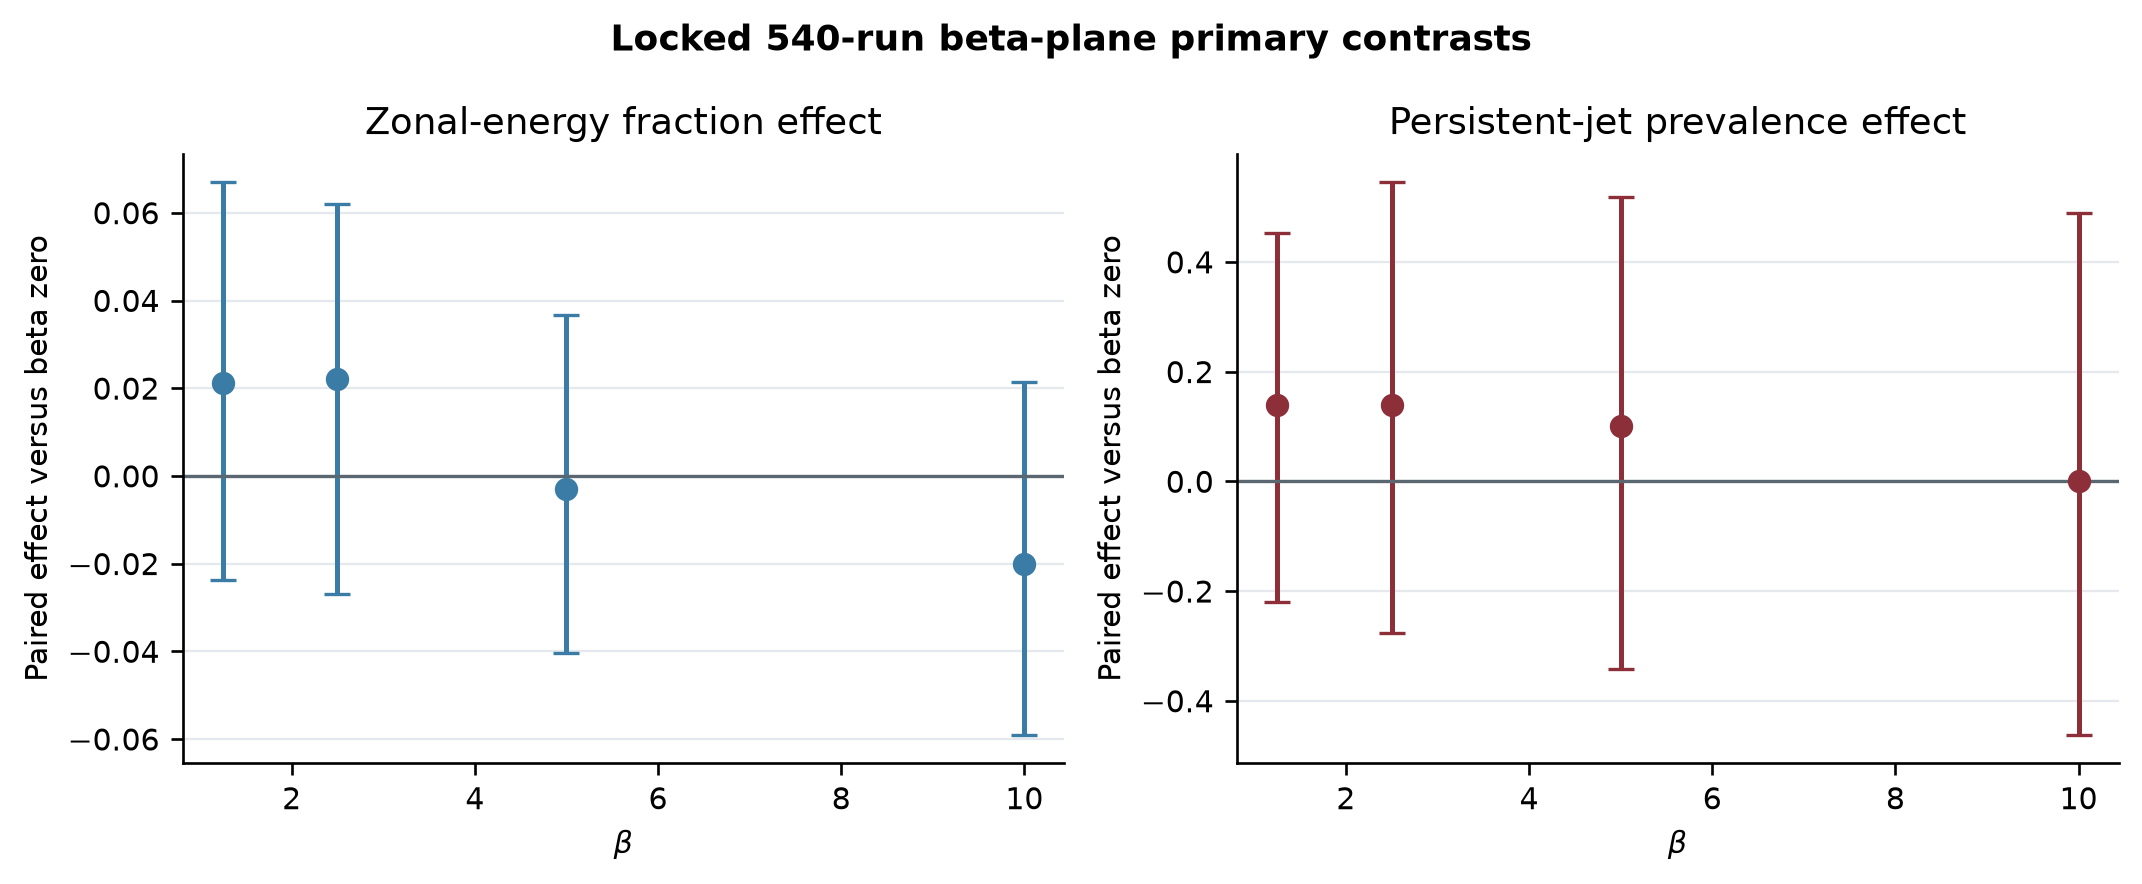
\includegraphics[width=\textwidth]{figures/review_beta_ablation.png}
  \caption{Primary effects from the locked 540-run beta-plane matrix. Error
  bars are simultaneous familywise 95 percent bootstrap intervals over twelve
  seed clusters. None of the four required $\beta=5,10$ contrasts passes.}
  \label{fig:beta-ablation}
\end{figure}

\begin{table}[htbp]
  \centering
  \caption{Required contrasts from the locked beta-plane production matrix.}
  \label{tab:beta-ablation-results}
  \small
  \begin{tabularx}{\textwidth}{>{\raggedright\arraybackslash}p{0.29\textwidth}YYYY}
    \toprule
    Metric & Effect & Lower bound & Upper bound & Decision \\
    \midrule
    Zonal-energy fraction at $\beta=5$ & -0.0030 & -0.0404 & 0.0368 & Not supported \\
Persistent-jet prevalence at $\beta=5$ & 0.1019 & -0.3426 & 0.5185 & Not supported \\
Zonal-energy fraction at $\beta=10$ & -0.0200 & -0.0592 & 0.0215 & Not supported \\
Persistent-jet prevalence at $\beta=10$ & 0.0000 & -0.4630 & 0.4885 & Not supported \\
\bottomrule

  \end{tabularx}
\end{table}
